%%%%%%%%%%%%%%%%%%%%%%%%%%%%%%%%%%%%%%%%%%%%%%%%%%%%%%%%%%%%
%%  This Beamer template was created by Cameron Bracken.
%%  Anyone can freely use or modify it for any purpose
%%  without attribution.
%%
%%  Last Modified: January 9, 2009
%%http://cameron.bracken.bz/beamer-template

\documentclass[xcolor=x11names,compress]{beamer}

%% General document %%%%%%%%%%%%%%%%%%%%%%%%%%%%%%%%%%
\usepackage{graphicx}
\usepackage{tikz}
\usetikzlibrary{decorations.fractals}
%%%%%%%%%%%%%%%%%%%%%%%%%%%%%%%%%%%%%%%%%%%%%%%%%%%%%%


%% Beamer Layout %%%%%%%%%%%%%%%%%%%%%%%%%%%%%%%%%%
\useoutertheme[subsection=false,shadow]{miniframes}
\useinnertheme{default}
\usefonttheme{serif}
\usepackage{palatino}

\setbeamerfont{title like}{shape=\scshape}
\setbeamerfont{frametitle}{shape=\scshape}

\setbeamercolor*{lower separation line head}{bg=DeepSkyBlue4} 
\setbeamercolor*{normal text}{fg=black,bg=white} 
\setbeamercolor*{alerted text}{fg=red} 
\setbeamercolor*{example text}{fg=black} 
\setbeamercolor*{structure}{fg=black} 
 
\setbeamercolor*{palette tertiary}{fg=black,bg=black!10} 
\setbeamercolor*{palette quaternary}{fg=black,bg=black!10} 

\renewcommand{\(}{\begin{columns}}
\renewcommand{\)}{\end{columns}}
\newcommand{\<}[1]{\begin{column}{#1}}
\renewcommand{\>}{\end{column}}
%%%%%%%%%%%%%%%%%%%%%%%%%%%%%%%%%%%%%%%%%%%%%%%%%%

\usepackage{tikz}
\usepackage{graphicx}
%\usepackage{sidecap}
\usepackage{caption}
\captionsetup[figure]{labelformat=empty}
\usepackage[utf8]{inputenc}
\usepackage{polski}
%\usepackage[polish]{babel}
\usepackage{multimedia}
\usepackage{media9}
\begin{document}


%%%%%%%%%%%%%%%%%%%%%%%%%%%%%%%%%%%%%%%%%%%%%%%%%%%%%%
%%%%%%%%%%%%%%%%%%%%%%%%%%%%%%%%%%%%%%%%%%%%%%%%%%%%%%
\section{\scshape Introduction}
\begin{frame}
\title{Wine classification based on their chemical analysis}
\subtitle{\begin{figure}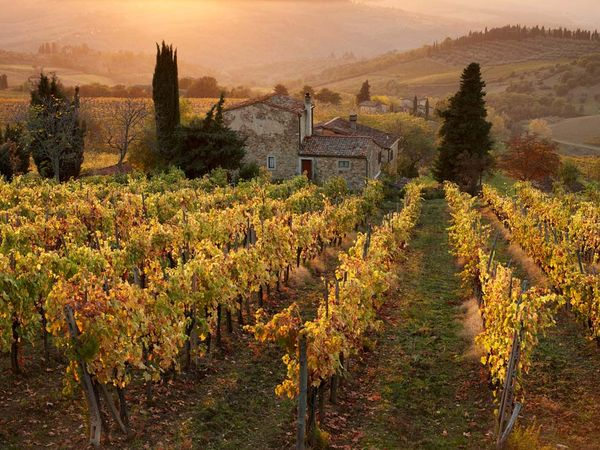
\includegraphics[width=0.6\textwidth]{winnica.jpg}  \caption{Adrianna Janik}  \end{figure}} 
\titlepage
\end{frame}

%%%%%%%%%%%%%%%%%%%%%%%%%%%%%%%%%%%%%%%%%%%%%%%%%%%%%%
%%%%%%%%%%%%%%%%%%%%%%%%%%%%%%%%%%%%%%%%%%%%%%%%%%%%%%
\section{\scshape Problem description}
\subsection{Data}
\begin{frame}{Data}
	UCI Machine Learning repository: \url{http://archive.ics.uci.edu/ml/datasets/Wine} \\
        Number of instances: 178 \\
	Number of attributes: 13 \\
	Attributes: \\
        \begin{itemize}

	\begin{columns}
	\begin{column}{0.5\textwidth}
		\item Alcohol 
		\item  Malic acid 
		\item  Ash  
		\item	Alcalinity of ash 
		\item	Magnesium 
		\item	Total phenols  
	\end{column}
	\begin{column}{0.5\textwidth}  %%<--- here
		\item	Flavanoids  
		\item	Nonflavanoid phenols  
		\item	Proanthocyanins 
		\item	Color intensity   
		\item	Hue 
		\item  OD280/OD315 of diluted wines  
		\item Proline
	\end{column}
	\end{columns}
	\end{itemize}	

\end{frame}
\begin{frame}{Box plots}
	\begin{columns}
	\column{\dimexpr\paperwidth-20pt}

	\begin{center}
%        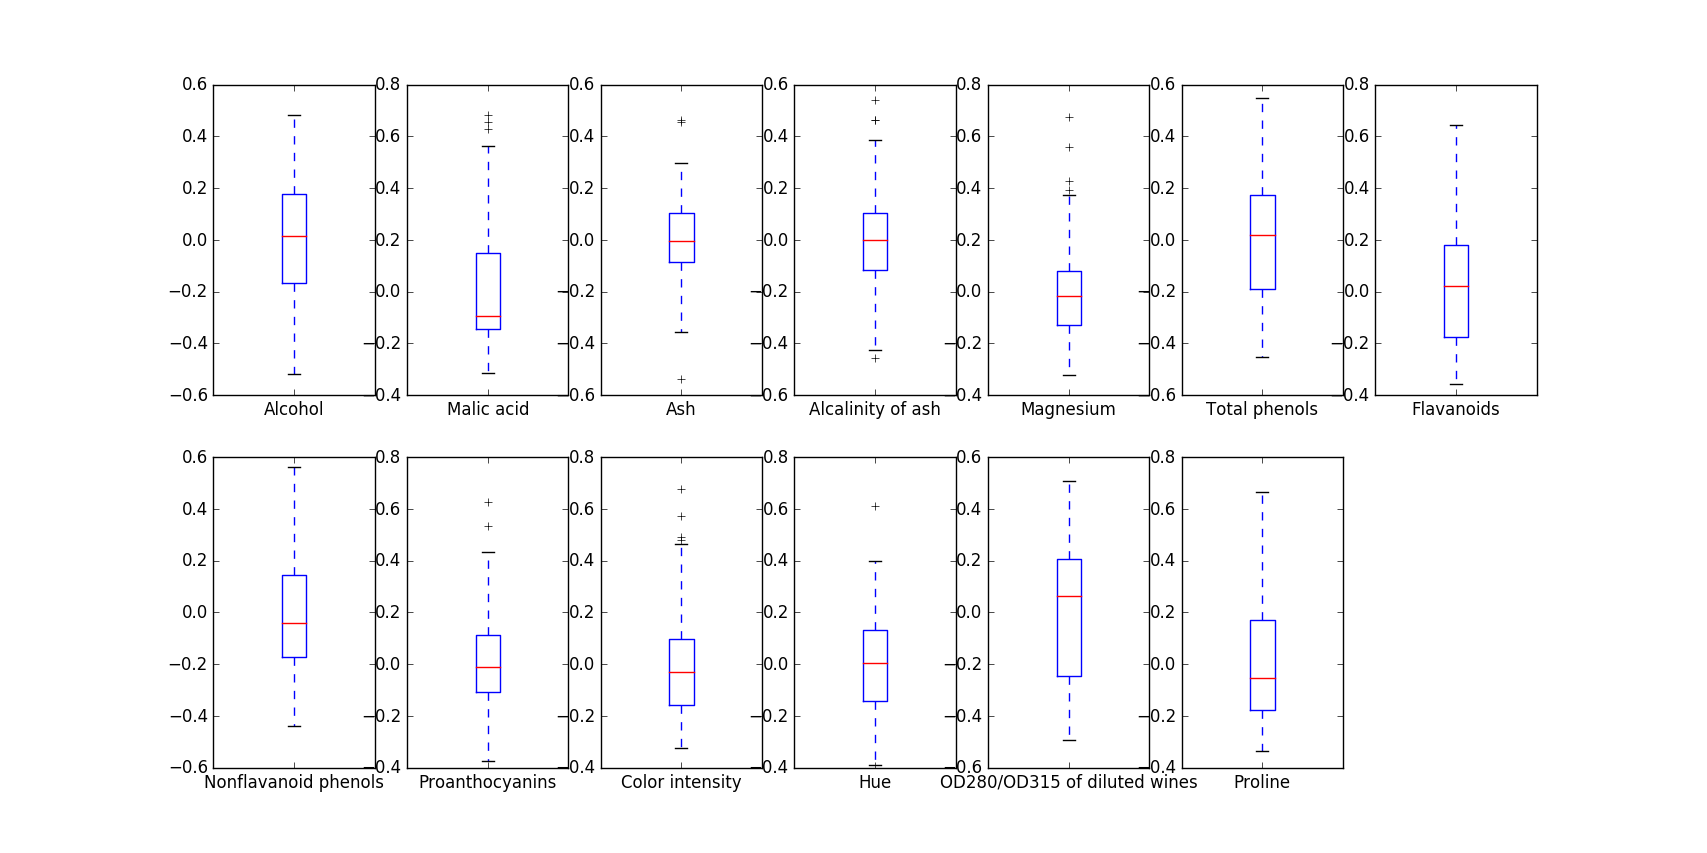
\includegraphics[width=1\textwidth]{box_chart.png}
        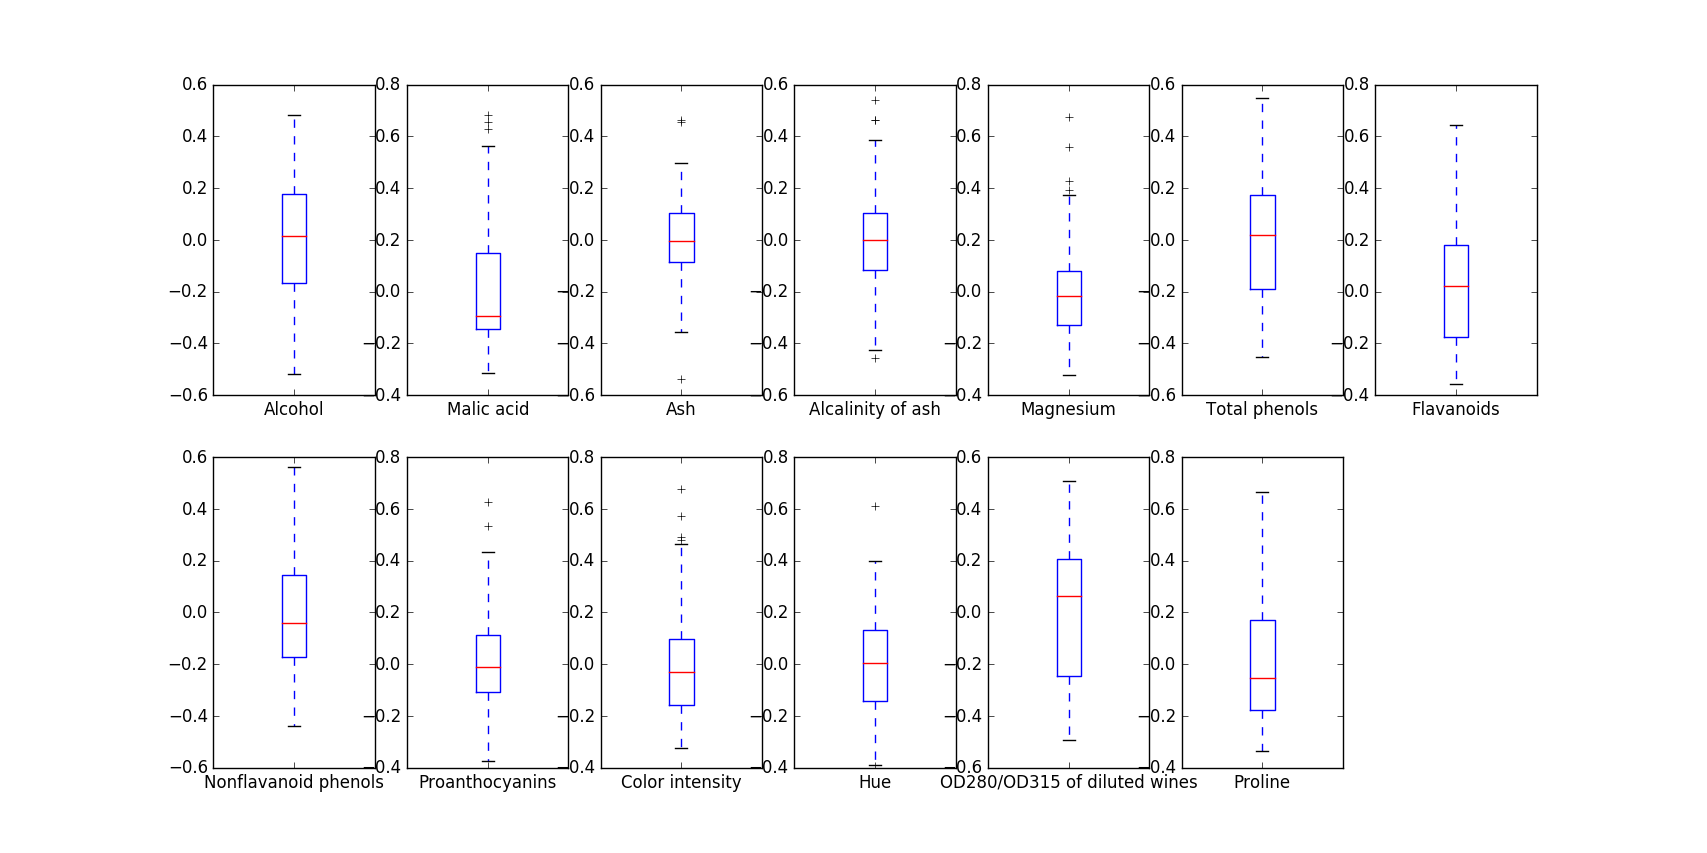
\includegraphics[width=360]{box_chart.png}

	\end{center}
        \end{columns}

\end{frame}
\begin{frame}{Histograms}
	\begin{columns}
	\column{\dimexpr\paperwidth-20pt}

        \begin{figure}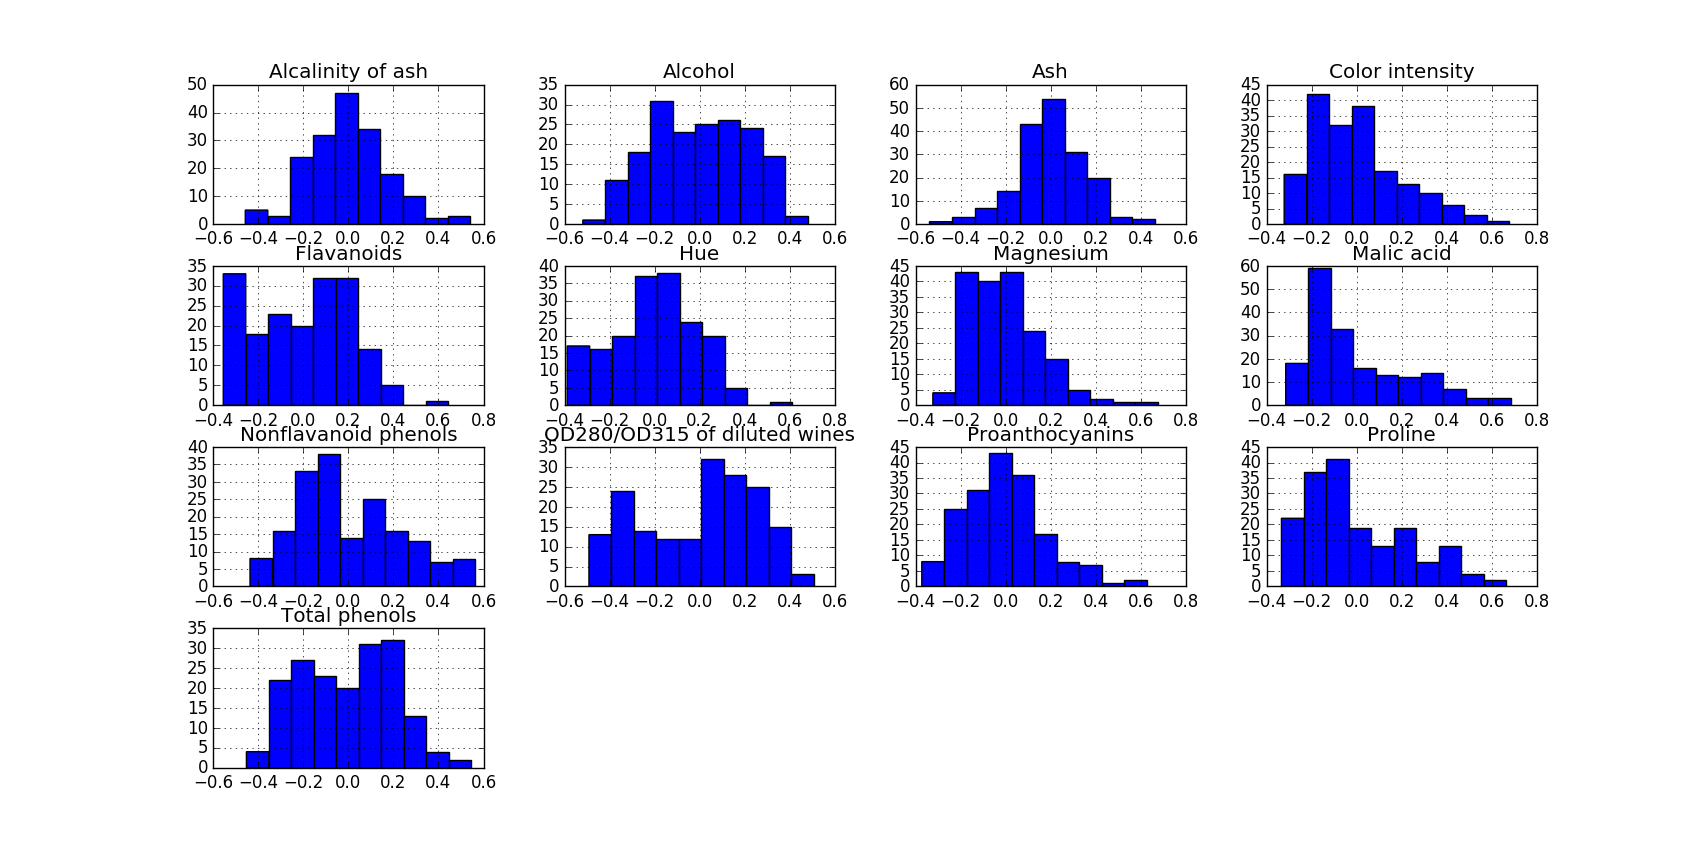
\includegraphics[width=1\textwidth]{hist_chart.png} \end{figure}
 \end{columns}

\end{frame}

\begin{frame}{Density charts}
	\begin{columns}
	\column{\dimexpr\paperwidth-20pt}

        \begin{figure}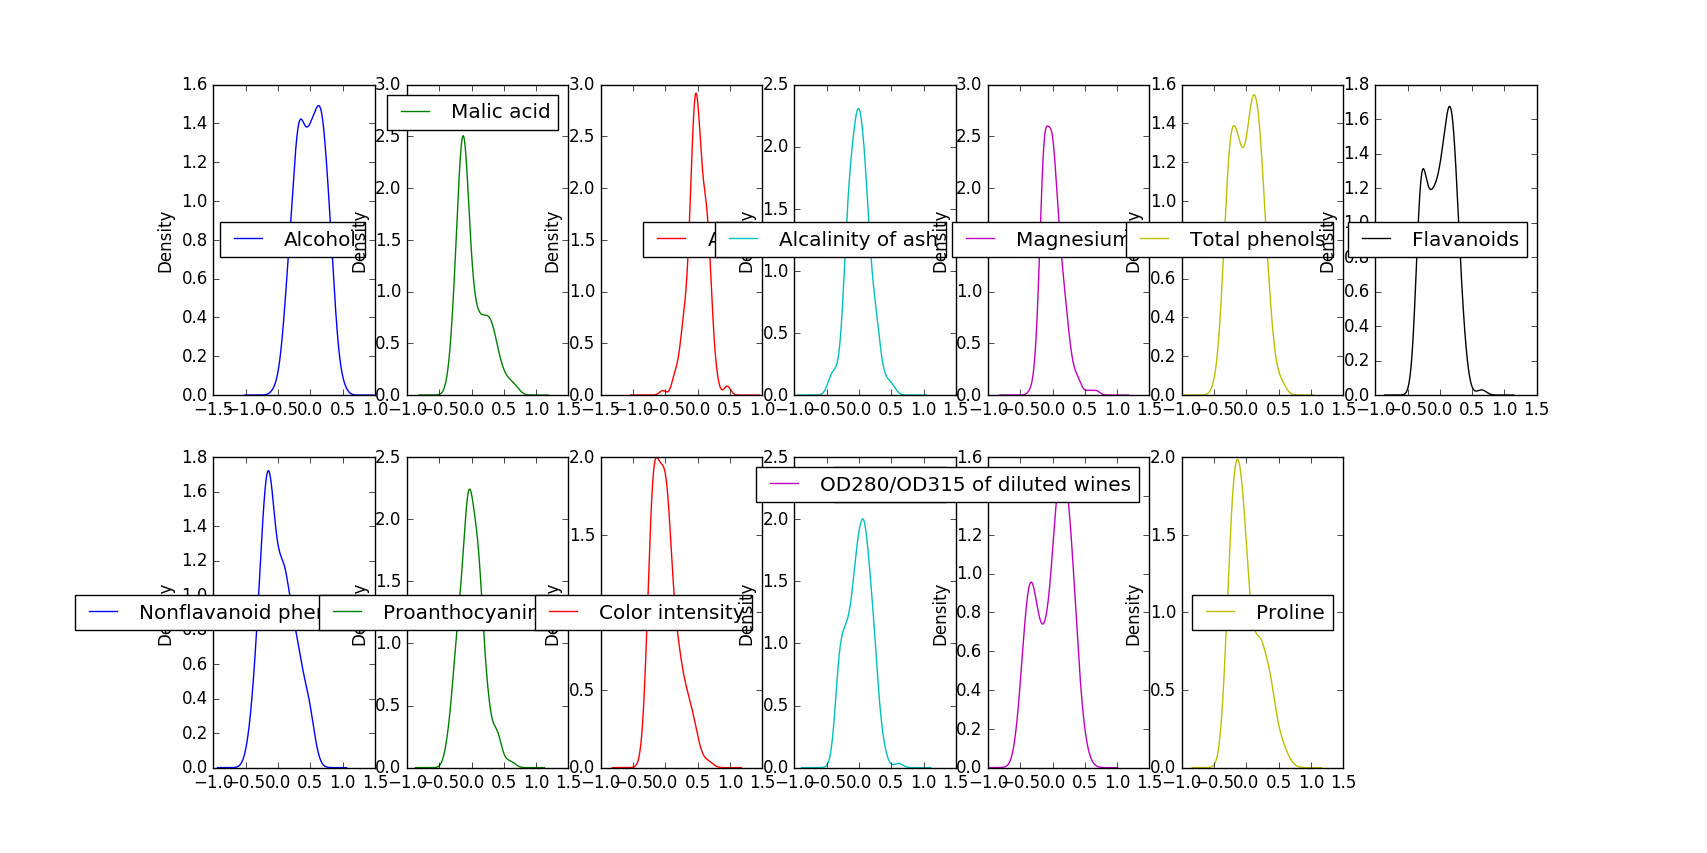
\includegraphics[width=1\textwidth]{density_chart.png} \end{figure}
 \end{columns}
\end{frame}

%\begin{frame}
%	\begin{columns}
%	\column{\dimexpr\paperwidth-20pt}
%
%        \begin{figure}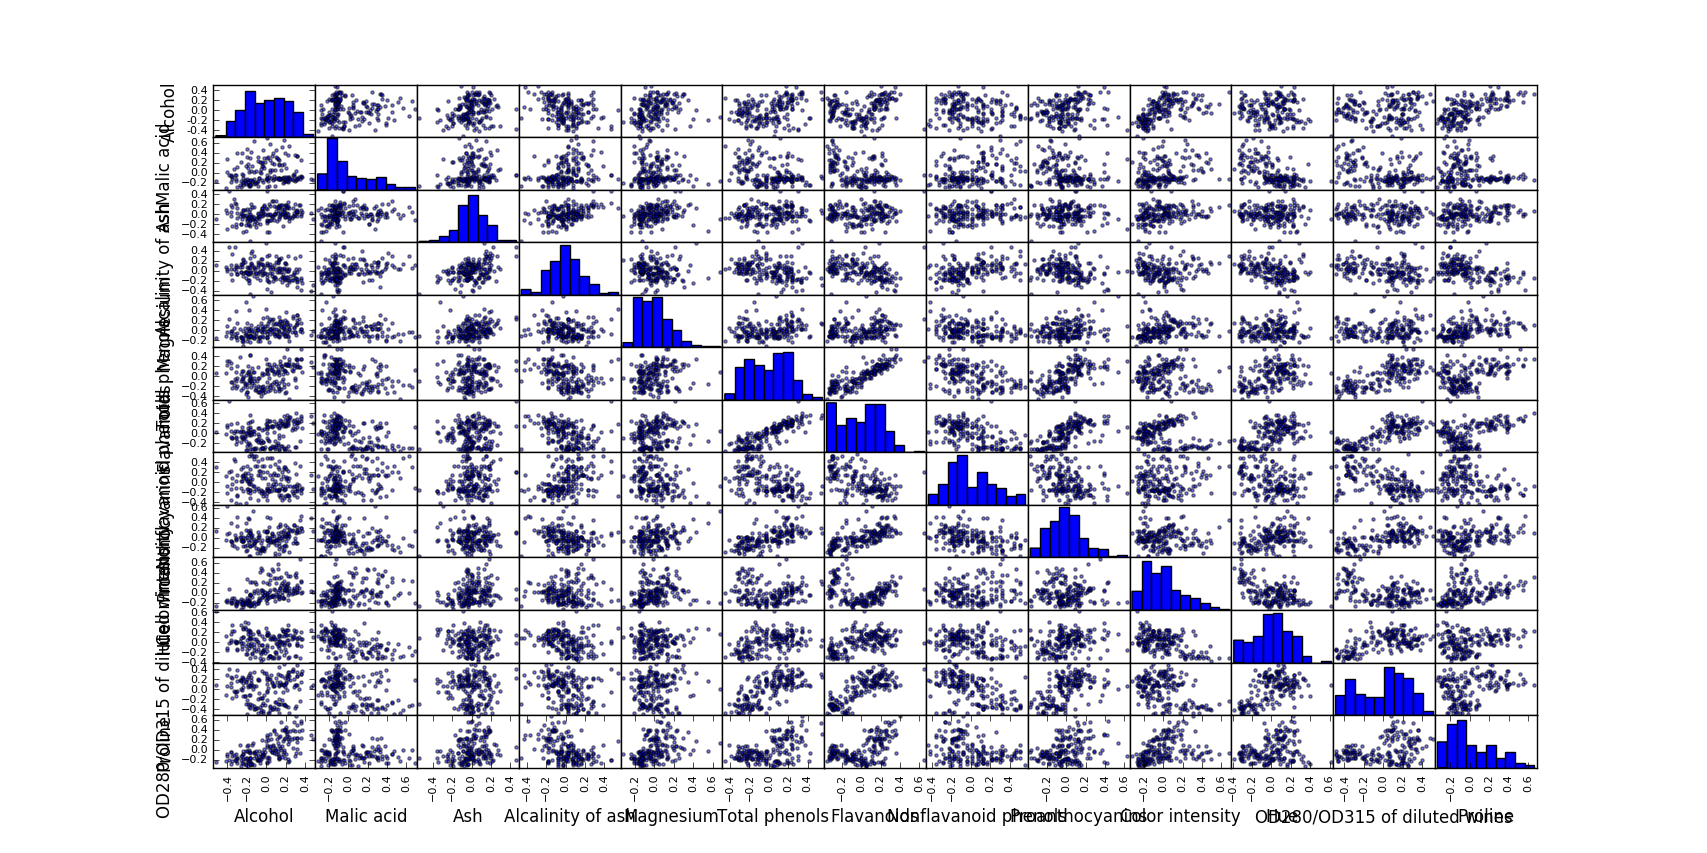
\includegraphics[width=1\textwidth]{scatter_matrix.png} \end{figure}
% \end{columns}
%
%\end{frame}

%%%%%%%%%%%%%%%%%%%%%%%%%%%%%%%%%%%%%%%%%%%%%%%%%%%%%%
%%%%%%%%%%%%%%%%%%%%%%%%%%%%%%%%%%%%%%%%%%%%%%%%%%%%%%
\section{\scshape Methodology}
\subsection{}
\begin{frame}{Normalization and data set division}
	$X_{norm} = \frac{x - \mu}{x_{max} -x_{min}}$ \\
	
    \begin{table}[t]
    \begin{tabular}{|l|c|c|}
      \hline 
      Class &  Instances & \%\\
      \hline 
      1 & 59 & 33\%\\
      \hline
      2 & 71 & 39\%\\
      \hline
      3 & 48 & 27\%\\
      \hline
    \end{tabular} \\
    \end{table}

training data set: 142 \\
validation data set: 36 \\
cross-validation: 10-fold \\

\end{frame}

\subsection{}
\begin{frame}{Analyzed algorithms}
	\begin{itemize}
	\item Logistic regression
	\item LDA
	\item K\dywiz nearest neighbors
	\item Decision tree
	\item Naive Bayes
	\item SVM
	\item Multilayer perceptron
	\item Logistic regression One vs all

\end{itemize}
\end{frame}

\begin{frame}{Linear discriminant analysis LDA}
        \begin{figure}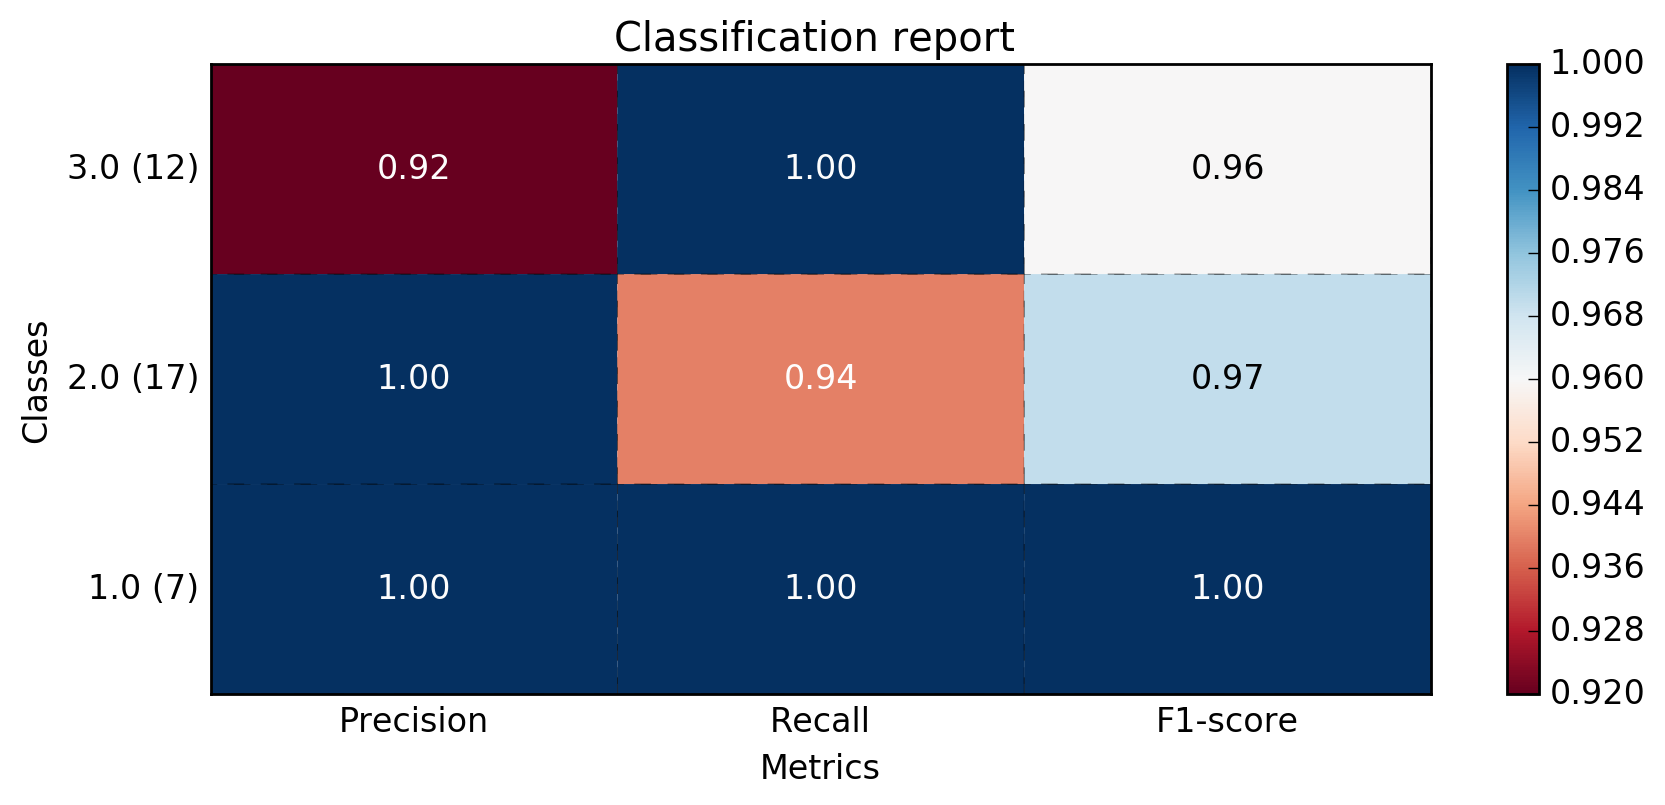
\includegraphics[width=1\textwidth]{lda.png} \end{figure}

\end{frame}

\begin{frame}{Multilayer perceptron MLP}
        \begin{figure}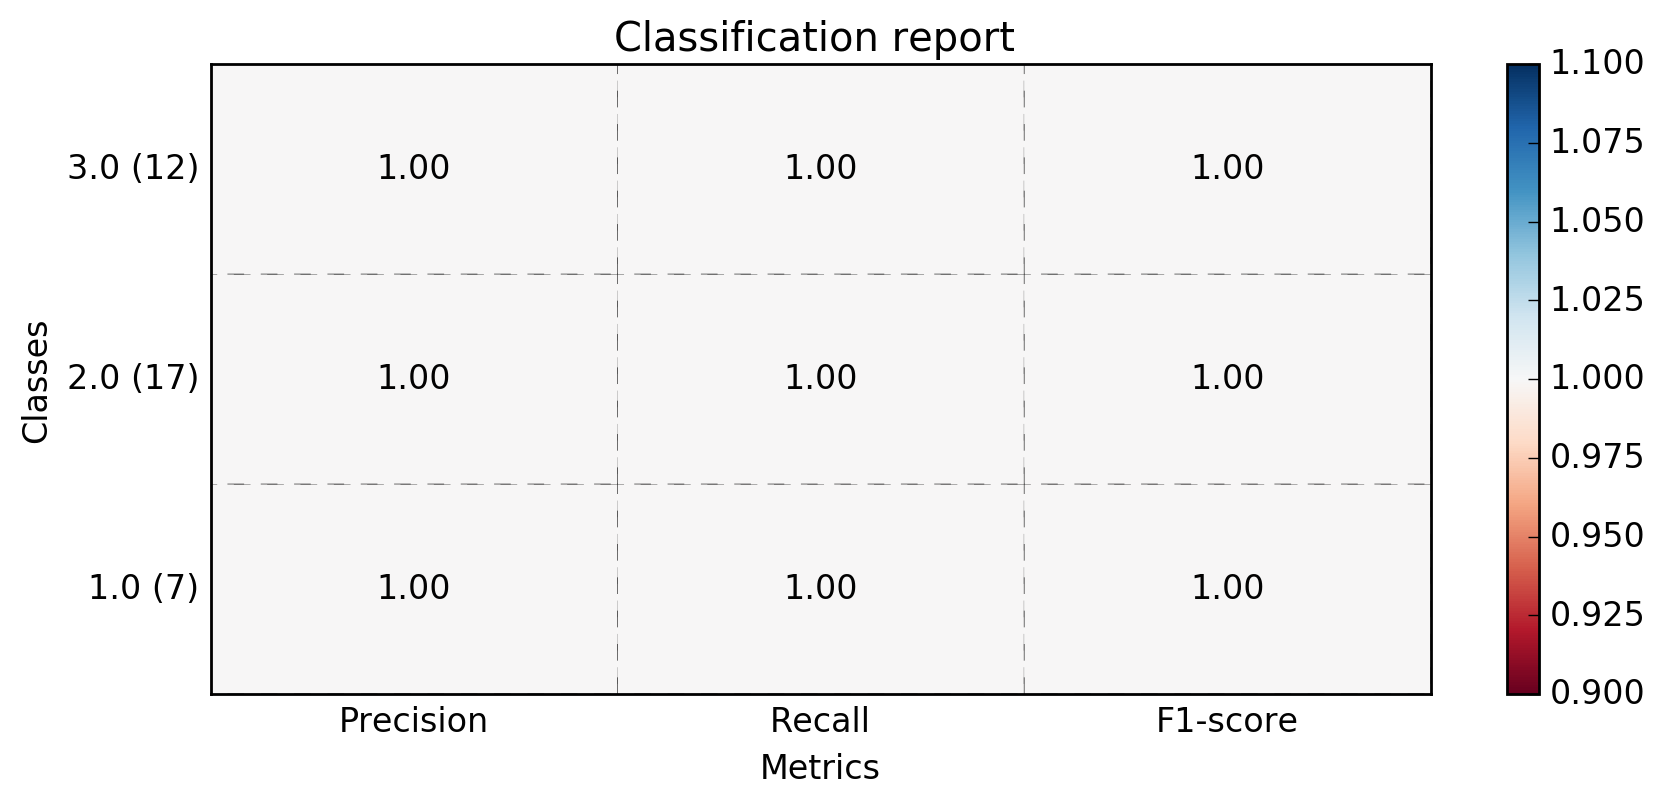
\includegraphics[width=1\textwidth]{mlp.png} \end{figure}

\end{frame}
\begin{frame}{Neural network structure}
	\begin{columns}
	\column{\dimexpr\paperwidth-20pt}

        \begin{figure}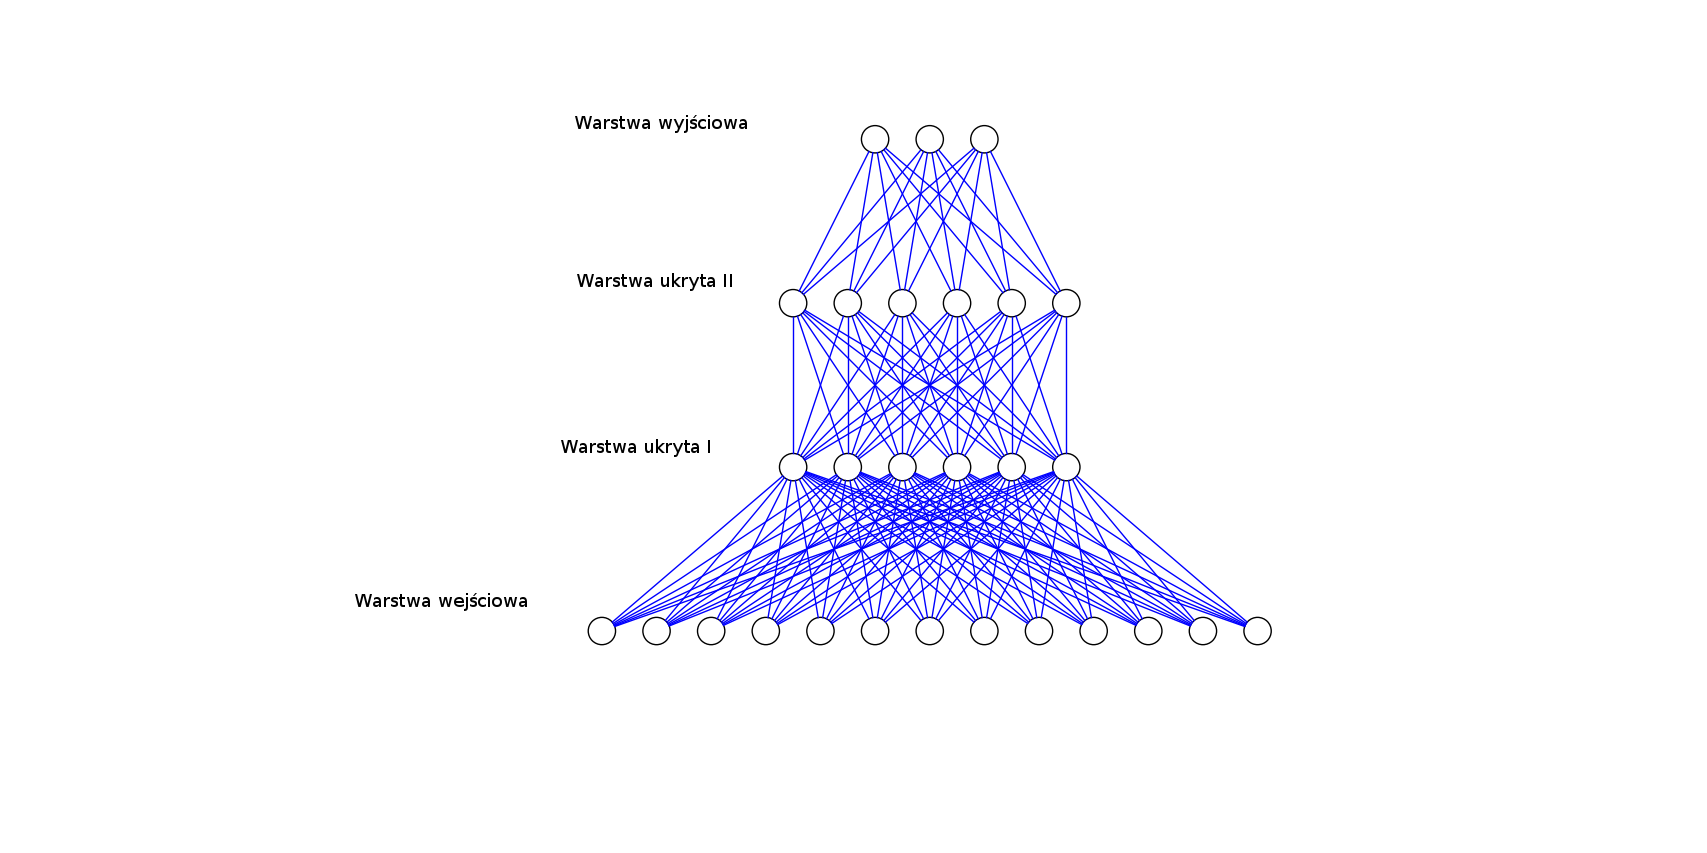
\includegraphics[width=400]{nn.png} \end{figure}
        \end{columns}
\end{frame}



\begin{frame}{Logistic regression - One vs all}
        \begin{figure}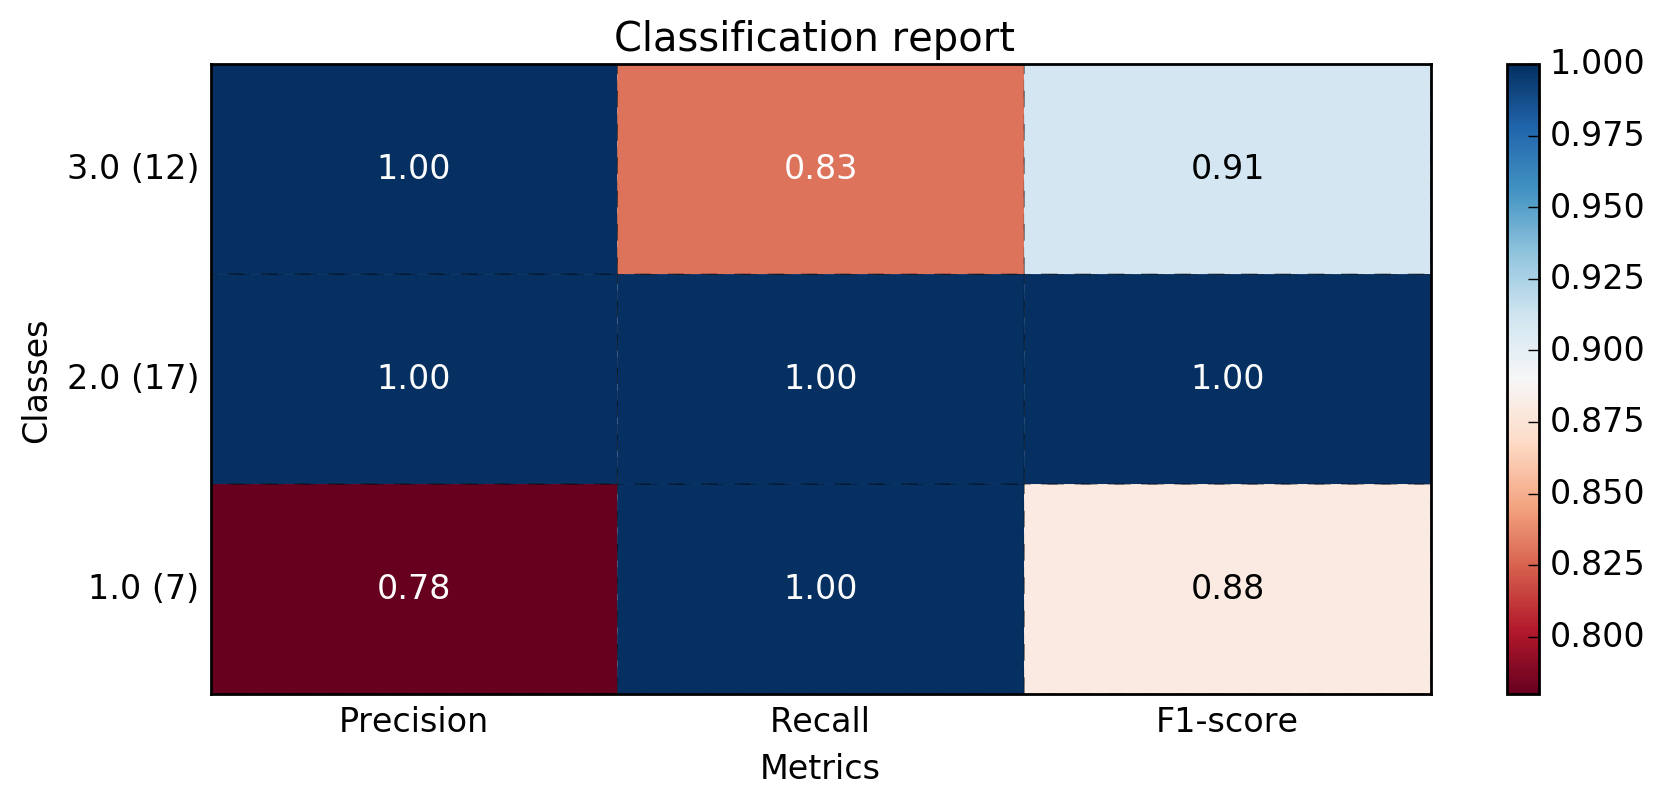
\includegraphics[width=1\textwidth]{one_vs_all.png} \end{figure}

\end{frame}

\subsection{Tools}
\begin{frame}{Tools}
	\begin{itemize}
	%	\item{Blender 2.68} %\begin{figure} 
\includegraphics[width=0.4\textwidth]{blender.png}  \end{figure}}
		\item{Python 2.7.12} %\begin{figure} 
\includegraphics[width=0.4\textwidth]{python.png}  \end{figure}}

		\item{libraries: numpy, matplotlib, scipy, scikit-learn
				
                    \begin{figure}
                    \centering
                    \begin{minipage}{.3\textwidth}
                    
\includegraphics[width=\linewidth]{python.png}
                    \label{fig:test1}
                    \end{minipage}\hfill
                    \begin{minipage}{.3\textwidth}
                    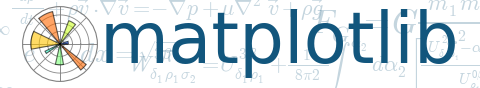
\includegraphics[width=\linewidth]{matplotlib.png}
                    \label{fig:test3}
                    \end{minipage}
                    \end{figure}			

		    \begin{figure}
		    \centring
                    \begin{minipage}{.3\textwidth}
                    
\includegraphics[width=\linewidth]{numpy.png}
                    \label{fig:test2}
                    \end{minipage}\hfill
 
		    \end{figure}

                    \begin{figure}
                    \centering
                    \begin{minipage}{.17\textwidth}
                    
\includegraphics[width=\linewidth]{scipy.png}
                    \label{fig:test1}
                    \end{minipage}\hfill
                    \begin{minipage}{.2\textwidth}
                    
\includegraphics[width=\linewidth]{scikit.png}
                    \label{fig:test2}
                    \end{minipage}\hfill

                   \end{figure}				
			}
	\end{itemize}
\end{frame}

%%%%%%%%%%%%%%%%%%%%%%%%%%%%%%%%%%%%%%%%%%%%%%%%%%%%%%
%%%%%%%%%%%%%%%%%%%%%%%%%%%%%%%%%%%%%%%%%%%%%%%%%%%%%%
\section{\scshape Results}
\subsection{}
\begin{frame}{Results}

    \begin{table}[t]
    \begin{tabular}{|l|c|c|}
      \hline 
      Algorithm &  result \\
      \hline
      MLP & 100\% \\
      \hline
      LDA & 98\% \\
      \hline
      LR & 95\% \\
      \hline
      NB & 94\% \\
      \hline
      SVM & 94\% \\
      \hline
      KNN & 92\% \\
      \hline
      CART & 91\% \\
      \hline
      LR One vs all & 85\% \\
      \hline
    \end{tabular} \\
    \end{table}
	
\end{frame}

\end{document}
